\apendice{Especificación de Requisitos}

\section{Introducción}

Este apéndice recoge los requisitos funcionales de la aplicación propuesta en este proyecto para evaluar la adopción de prácticas ágiles en repositorios de GitHub utilizados por estudiantes para realizar diversos trabajos como, por ejemplo, Trabajos de Fin de Grado (TFG). Se incluyen los casos de uso posibles que podrá tener un usuario de la aplicación desarrollada, junto a tablas y diagramas que ayuden a comprender los mismos. Los casos de uso comprenderán cierto número de requisitos funcionales y no funcionales, listados y explicados más adelante en este apartado para especificar claramente todas las formas que tiene el usuario de interactuar con el software propuesto. Además se incluirá el listado de objetivos generales del proyecto para ayudar a contextualizar tanto los casos de uso como los requisitos funcionales.

\section{Objetivos generales}
La visión general de este proyecto abarca los objetivos descritos a continuación:

\begin{itemize}

\item \textbf{Análisis de métricas de calidad de proceso de software de los repositorios}: La aplicación web analiza detalladamente todas las métricas de calidad de proceso y características que pueden resultar útiles de un repositorio durante el proceso de desarrollo de software.

\item \textbf{Ajuste temporal del análisis}: Consiste en la posibilidad de ajustar distintos parámetros temporales del análisis para elegir en qué etapas del desarrollo se analizarán los repositorios.

\item \textbf{Comparación de las métricas de calidad de proceso obtenidas de los repositorios de referencia}: La aplicación es capaz de, dadas todas las medidas de calidad de proceso de los repositorios que el usuario ha elegido como referencia, compararlas para ofrecer al usuario una visualización clara de los diferentes valores de estas medidas en los distintos repositorios.

\item \textbf{Prácticas ágiles y medidas de repositorios}: La aplicación utiliza las definiciones de prácticas ágiles recogidas en \cite{agileSubwayMap} para presentar los resultados al usuario tras analizar el repositorio.

\item \textbf{Asistencia a estudiantes}: Se pueden utilizar otros TFGs públicos realizados en la Universidad de Burgos como casos de estudio, introduciéndolos en la aplicación y que estos sirvan como referencia para los estudiantes a la hora de realizar sus propios TFG.

\end{itemize}

\section{Catálogo de requisitos}

\subsection{Requisitos funcionales}
A continuación se puede observar un listado de todos los requisitos funcionales considerados para la aplicación realizada en este proyecto.

\begin{itemize}
    \item \textbf{RF-01} – Creación una cuenta para usar la aplicación.
    
    \item \textbf{RF-02} – Entrada al perfil creado iniciando sesión.
    
    \item \textbf{RF-03} – Salida  del perfil creado cerrando sesión.
    
    \item \textbf{RF-04} – Cambio de la contraseña del perfil de la cuenta creada.
    
    \item \textbf{RF-05} – Cambio del idioma de la interfaz de usuario de la aplicación.
    
    \item \textbf{RF-06} – Introducción y validación de URLs de repositorios.
    
    \item \textbf{RF-07} – Elección del número de días para realizar el cálculo de las medidas de calidad temporales.
    
    \item \textbf{RF-08} – Elección del ámbito termporal de extracción de medidas de calidad de proceso de los repositorios.
    
    \item \textbf{RF-09} – Elección del tipo de intervalos de tiempo a usar para extraer las medidas de calidad de proceso de los repositorios introducidos.
    
    \item \textbf{RF-10} – Ajuste de los intervalos de tiempo específicos para elegir de qué momento en el tiempo de vida de los repositorios se extraerán las medidas de calidad de proceso.
    
    \item \textbf{RF-11} – Carga de grupos de repositorios usados como fuente de referencia en la aplicación con anterioridad.
    
    \item \textbf{RF-12} – Borrado de grupos de repositorios usados como fuente de referencia en la aplicación con anterioridad.
    
    \item \textbf{RF-13} – Visualización de la evaluación de la aplicación de prácticas ágiles por parte del repositorio a evaluar.
    
    \item \textbf{RF-14} – Visualización de la comparación de los valores numéricos de las medidas de calidad de proceso entre el repositorio a analizar y los repositorios de referencia.
\end{itemize}

\subsection{Requisitos no funcionales}

Continuando los requisitos del proyecto, más adelante se encuentra un listado de todos los requisitos no funcionales considerados para la aplicación realizada en este proyecto.

\begin{itemize}
    \item \textbf{RNF-01} Modularidad

    \item \textbf{RNF-02} Usabilidad

    \item \textbf{RNF-03} Reusabilidad

    \item \textbf{RNF-04} Separación entre frontend y backend

    \item \textbf{RNF-05} Validaciones informativas

    \item \textbf{RNF-06} Navegación intuitiva
\end{itemize}

\section{Especificación de requisitos}

\subsection{Requisitos funcionales}

A continuación se describen de forma detallada los requisitos funcionales del sistema.

\begin{itemize}

    \item *{RF-01 – Creación de una cuenta de usuario}
    El sistema debe permitir a los usuarios crear una cuenta personal mediante un formulario de registro. Esta funcionalidad es necesaria para garantizar la personalización de la experiencia, el almacenamiento de configuraciones y el acceso a funcionalidades avanzadas, como la carga de repositorios de referencia o la consulta del historial de análisis realizados; además de garantizar seguridad y control de acceso a la aplicación.
    
    \item*{RF-02 – Inicio  de sesión}
    Los usuarios registrados deben poder iniciar sesión en el sistema para acceder a sus perfiles y funcionalidades asociadas mediante un nombre de usuario único y una contraseña que se almacenará encriptada para garantizar la seguridad del almacenaje de perfiles de usuario en la base de datos.
    
    \item*{RF-03 – Cierre de sesión}
    Los usuarios pueden cerrar sesión de forma segura al finalizar su uso, tanto para finalizar de forma segura su actividad o cambiar de cuenta por diferentes motivos como el uso de varias cuentas personalizadas con diferentes ajustes y/o grupos de repositorios almacenados.
    
    \item*{RF-04 – Cambio de contraseña}
    El sistema debe permitir a los usuarios modificar la contraseña de su cuenta en cualquier momento, con el fin de mantener la seguridad y el control sobre su acceso. El proceso debe incluir medidas de validación para evitar contraseñas débiles o inseguras.
    
    \item*{RF-05 – Cambio de idioma de la interfaz}
    La interfaz de la aplicación debe ser multilingüe, permitiendo a los usuarios seleccionar el idioma que prefieran entre las opciones disponibles. Esto contribuye a la internacionalización del software, mejora la accesibilidad y facilita su uso en contextos internacionales o multilingües.
    
    \item*{RF-06 – Introducción y validación de URLs de repositorios}
    El sistema debe permitir a los usuarios introducir la URL de uno o varios repositorios públicos de GitHub. La aplicación validará que las URLs introducidas sean correctas, que los repositorios estén disponibles y que se pueda acceder a ellos para su análisis para informar al usuario de que está introduciendo repositorios válidos y de manera correcta.
    
    \item*{RF-07 – Selección del número de días para métricas temporales}
    El sistema debe permitir al usuario definir un número de días a considerar como ventana temporal para el cálculo de medidas de calidad de proceso relacionadas con medias. Esta opción permite realizar análisis adaptados a periodos de mayor o menor longitud de actividad dentro del proyecto.
    
    \item*{RF-08 – Selección del ámbito temporal del análisis}
    Los usuarios podrán definir si los repositorios se analizarán al completo, lo cual abarcaría todo su tiempo de vida desde el primer \textit{commit} hasta el último, o por intervalos de tiempo ajustables.
    
    \item*{RF-09 – Selección del tipo de intervalos de tiempo}
    El sistema debe ofrecer la posibilidad de seleccionar el tipo de intervalo temporal para el análisis, ya sean intervalos relativos, que abarquen cuartos de la vida del repositorio, o intervalos absolutos que equivalgan a meses de vida. Esta opción facilita la visualización de tendencias y eficiencia de trabajo en distintas fases del desarrollo de software.
    
    \item*{RF-10 – Ajuste manual de intervalos de tiempo}
    Además de seleccionar el tipo de intervalo, el usuario podrá definir manualmente los intervalos exactos de tiempo que desea analizar (Por ejemplo el primer y segundo cuarto, lo cual es equivalente a la primera mitad del repositorio para los intervalos relativos, o del tercer al sexto mes de vida del repositorio para los intervalos absolutos). Esta funcionalidad avanzada permite focalizar el análisis en momentos clave del desarrollo del proyecto.
    
    \item*{RF-11 – Carga de grupos de repositorios de referencia}
    La aplicación debe permitir al usuario cargar grupos de repositorios previamente definidos como referencia. Esto permite al usuario repetir comparaciones o realizar comparaciones muy similares evitando el tiempo de extracción de medidas de calidad de proceso.
    
    \item*{RF-12 – Eliminación de grupos de referencia cargados*}
    El usuario también debe tener la posibilidad de eliminar grupos de repositorios de referencia previamente cargados, con el fin de mantener organizada su área de trabajo y adaptar el análisis a nuevos contextos o criterios de comparación.
    
    \item*{RF-13 – Visualización de la evaluación de prácticas ágiles}
    Una vez realizado el análisis, el sistema debe mostrar una evaluación del repositorio analizado en función de su cumplimiento de buenas prácticas ágiles. Esta evaluación debe representarse de forma clara y comprensible en forma de reglas que indiquen visualmente en qué aspectos se usan de forma sólida las metodologías ágiles y en qué aspectos hay opción de mejora.
    
    \item*{RF-14 – Comparación con repositorios de referencia}
    La aplicación debe permitir comparar los valores de todas las métricas extraídas del repositorio analizado con los correspondientes valores de los repositorios de referencia seleccionados. Esta comparación se visualizará mediante listas que ayuden a respaldar la evaluación del uso de prácticas ágiles en los repositorios.
\end{itemize}

\subsection{Requisitos no funcionales}

A continuación se describen de forma detallada los requisitos no funcionales del sistema.

\begin{itemize}

    \item*{RNF-01 – Modularidad}
    La aplicación debe estar diseñada utilizando una arquitectura modular basada en componentes reutilizables. Debe ser compatible con patrones de diseño modernos y fácil de escalar o modificar por partes sin afectar al conjunto total del software. Esta estructura permite que futuras modificaciones o ampliaciones (como la adición de nuevas métricas o funcionalidades) se integren de forma controlada y sencilla.
    
    \item*{RNF-02 – Usabilidad}
    La interfaz debe ser intuitiva, clara y fácil de usar. Los formularios deben presentar instrucciones comprensibles, validaciones dinámicas y retroalimentación inmediata ante errores o acciones del usuario. Se prioriza un diseño simple y directo que permita a usuarios no técnicos comprender la aplicación sin curva de aprendizaje.
    
    \item*{RNF-03 – Reusabilidad}
    El código debe seguir principios como DRY (Don’t Repeat Yourself) y SOLID, en particular el principio Open/Closed, que facilita la extensión de funcionalidades sin modificar el núcleo existente. La organización del código promueve la reutilización de servicios, componentes y lógica, favoreciendo la eficiencia en el desarrollo y la reducción de errores.
    
    \item*{RNF-04 –Separación entre frontend y backend}
    El sistema debe mantener una separación estricta entre las capas de presentación (frontend) y lógica de negocio (backend), utilizando servicios HTTP para el intercambio de datos de forma asíncrona. Esto mejora la escalabilidad y permite gestionar respuestas y errores de forma controlada desde la interfaz.
    
    \item*{RNF-05 – Validaciones informativas}
    Los formularios deben incorporar validación reactiva utilizando sistemas de formularios y alertas, proporcionando retroalimentación inmediata al usuario en caso de errores o datos incompletos. Esto reduce la frustración del usuario y mantiene informado al mismo, y además mejora la precisión y seguridad de los datos introducidos.
    
    \item*{RNF-06 – Navegación intuitiva}
    La aplicación debe organizar sus funcionalidades de forma jerárquica, utilizando tabs, rutas y botones de navegación claros que guíen al usuario durante el análisis. Los componentes de navegación deben ser reutilizables y consistentes en toda la aplicación para facilitar el acceso rápido a las diferentes secciones.

\end{itemize}

\subsection{Casos de uso}

En esta sección se presentan los diferentes casos de uso que encapsulan los requisitos previamente definidos, con el fin de cumplir los objetivos funcionales y no funcionales establecidos para la aplicación. Cada uno de estos casos de uso describe una interacción específica entre los actores del sistema (en el caso de esta aplicación: el usuario, el backend y el frontend) y sus funcionalidades principales, proporcionando así una visión clara de cómo se espera que los usuarios interactúen con la aplicación. Esto permite no solo una mejor comprensión de las funcionalidades esenciales del sistema, sino también una base sólida para futuras etapas de diseño e implementación. La Figura \ref{fig:Diagrama-casos-de-uso} ilustra de manera general todos los casos de uso identificados, organizando visualmente las relaciones entre los actores principales y las funcionalidades del sistema, lo cual facilita su análisis y validación.

\begin{figure}[H]
\centering
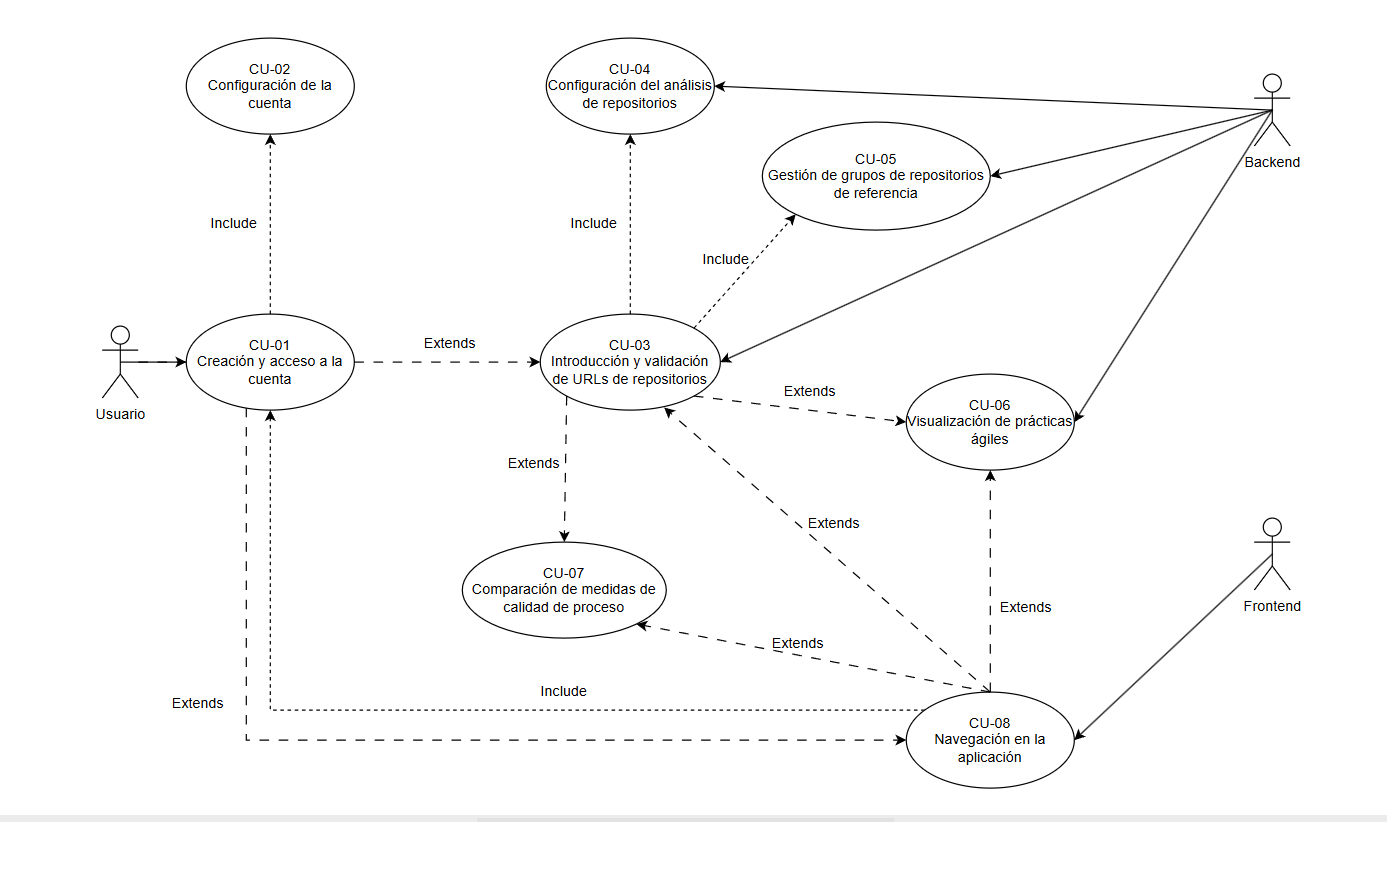
\includegraphics[width=0.8\textwidth]{img/Diagrama-casos-de-uso.png}
\caption{Diagrama de casos de uso general}
\label{fig:Diagrama-casos-de-uso}
\end{figure}

% Caso de Uso 1 -> Creación y acceso a la cuenta
\clearpage
\begin{table}[p]
	\centering
	\begin{tabularx}{\linewidth}{ p{0.21\columnwidth} p{0.71\columnwidth} }
        \toprule
        \textbf{CU-1}    & \textbf{Creación y acceso a la cuenta} \\
        \toprule
        \textbf{Versión}              & 1.0 \\
        \textbf{Autor}                & Lucas Olmedo Diéz \\
        \textbf{Requisitos asociados} & RF-01, RF-02 \\
        \textbf{Descripción}          & Permite al usuario crear una cuenta y acceder a la aplicación mediante inicio de sesión. \\
        \textbf{Precondición}         & El usuario debe introducir un usuario único y una contraseña válida \\
        \textbf{Acciones}             &
        \begin{enumerate}
            \def\labelenumi{\arabic{enumi}.}
            \tightlist
            \item El usuario accede a la página de registro o inicio de sesión.
            \item El usuario introduce los datos necesarios (usuario y contraseña).
            \item El sistema verifica la validez de los datos.
            \item El sistema registra al usuario o permite el acceso según corresponda.
        \end{enumerate}\\
        \textbf{Postcondición}        & El usuario ha creado una cuenta o ha accedido a su perfil. \\
        \textbf{Excepciones}          & Datos incorrectos o cuenta inexistente/ya registrada. \\
        \textbf{Importancia}          & Alta \\
        \bottomrule
    \end{tabularx}
    \caption{CU-1 Creación y acceso a la cuenta.}
\end{table}

% Caso de Uso 2 -> Configuración de la cuenta
\clearpage
\begin{table}[p]
    \centering
    \begin{tabularx}{\linewidth}{ p{0.21\columnwidth} p{0.71\columnwidth} }
        \toprule
        \textbf{CU-2}    & Configuración de la cuenta \\
        \midrule
        \textbf{Versión}              & 1.0 \\
        \textbf{Autor}                & Lucas Olmedo Diéz \\
        \textbf{Requisitos asociados} & RF-02, RF-03 \\\
        \textbf{Descripción}          & Permite al usuario cambiar la contraseña y modificar el idioma de la aplicación. \\
        \textbf{Precondición}         & El usuario debe haber iniciado sesión. \\
        \textbf{Acciones}             &
        \begin{enumerate}
            \def\labelenumi{\arabic{enumi}.}
            \tightlist
            \item El usuario accede a la sección de configuración.
            \item Selecciona cambiar contraseña o idioma.
            \item El sistema valida y aplica los cambios.
        \end{enumerate}\\
        \textbf{Postcondición}        & Se actualizan las preferencias del usuario. \\
        \textbf{Excepciones}          & \\
        \textbf{Importancia}          & Media \\
        \bottomrule
    \end{tabularx}
    \caption{CU-2 Configuración de la cuenta.}
\end{table}

% Caso de Uso 3 -> Introducción y validación de URLs
\clearpage
\begin{table}[p]
    \centering
    \begin{tabularx}{\linewidth}{ p{0.21\columnwidth} p{0.71\columnwidth} }
        \toprule
        \textbf{CU-3}    & Introducción y validación de URLs de repositorios \\
        \midrule
        \textbf{Versión}              & 1.0 \\
        \textbf{Autor}                & Lucas Olmedo Diéz \\
        \textbf{Requisitos asociados} & RF-04 \\
        \textbf{Descripción}          & Permite al usuario introducir URLs de repositorios GitHub y valida su formato y accesibilidad. \\
        \textbf{Precondición}         & El usuario ha iniciado sesión. \\
        \textbf{Acciones}             &
        \begin{enumerate}
            \def\labelenumi{\arabic{enumi}.}
            \tightlist
            \item El usuario introduce una o varias URLs.
            \item El sistema valida la estructura y el acceso.
            \item Se informa al usuario del resultado.
        \end{enumerate}\\
        \textbf{Postcondición}        & Se aceptan o rechazan las URLs introducidas. \\
        \textbf{Excepciones}          & URL malformada o repositorio no accesible. \\
        \textbf{Importancia}          & Alta \\
        \bottomrule
    \end{tabularx}
    \caption{CU-3 Introducción y validación de URLs de repositorios.}
\end{table}

% CU-4: Configuración del análisis de repositorios
\clearpage
\begin{table}[p]
    \centering
    \begin{tabularx}{\linewidth}{ p{0.21\columnwidth} p{0.71\columnwidth} }
        \toprule
        \textbf{CU-4} & Configuración del análisis de repositorios \\
        \midrule
        \textbf{Versión} & 1.0 \\
        \textbf{Autor} & Lucas Olmedo Díez \\
        \textbf{Requisitos asociados} & RF-05, RF-06, RF-07,\ RF-08 \\
        \textbf{Descripción} & Permite al usuario configurar cómo se analizarán los datos del repositorio: intervalos absolutos o relativos, número de días para calcular las métricas temporales, períodos de los intervalos. \\
        \textbf{Precondición} & El usuario debe haber elegido la opción de "Analizar por intervalos de tiempo". \\
        \textbf{Acciones} &
        \begin{enumerate}
            \def\labelenumi{\arabic{enumi}.}
            \tightlist
            \item El usuario selecciona si desea usar fechas absolutas o relativas.
            \item Ajusta manualmente los intervalos de fechas específicos.
            \item Elige el tipo de intervalos para segmentar la información.
            \item (Opcional) Se cambia el númerod e días usado para obtener métricas de calidad temporales.
        \end{enumerate}\\
        \textbf{Postcondición} & El sistema ha almacenado la configuración de análisis para ser utilizada en el cálculo de métricas. \\
        \textbf{Excepciones} & Intervalos inválidos, número de días no válido, configuración incompleta. \\
        \textbf{Importancia} & Alta \\
        \bottomrule
    \end{tabularx}
    \caption{CU-4 Configurar análisis del repositorio}
\end{table}

% CU-5: Gestión de grupos de repositorios de referencia
\clearpage
\begin{table}[p]
    \centering
    \begin{tabularx}{\linewidth}{ p{0.21\columnwidth} p{0.71\columnwidth} }
        \toprule
        \textbf{CU-5} & Gestión de grupos de repositorios de referencia \\
        \midrule
        \textbf{Versión} & 1.0 \\
        \textbf{Autor} & Lucas Olmedo Díez \\
        \textbf{Requisitos asociados} & RF-09, RF-10 \\
        \textbf{Descripción} & Permite al usuario cargar o borrar grupos de repositorios previamente guardados para usarlos como referencia comparativa en los análisis. \\
        \textbf{Precondición} & El usuario debe haber hecho algún análisis previo con el que se guardaron repositorios de referencia. \\
        \textbf{Acciones} &
        \begin{enumerate}
            \def\labelenumi{\arabic{enumi}.}
            \tightlist
            \item El usuario accede a la sección de gestión de repositorios guardados.
            \item Selecciona un grupo de repositorios guardado previamente y lo carga.
            \item (Opcional) Elimina uno o más grupos guardados si lo desea.
        \end{enumerate}\\
        \textbf{Postcondición} & Los grupos seleccionados han sido cargados o eliminados exitosamente. \\
        \textbf{Excepciones} & No hay grupos guardados disponibles o error en la carga/borrado. \\
        \textbf{Importancia} & Media \\
        \bottomrule
    \end{tabularx}
    \caption{CU-5 Gestionar grupos de repositorios de comparación}
\end{table}

% CU-6: Visualización de prácticas ágiles
\clearpage
\begin{table}[p]
    \centering
    \begin{tabularx}{\linewidth}{ p{0.21\columnwidth} p{0.71\columnwidth} }
        \toprule
        \textbf{CU-6} & Visualización de prácticas ágiles \\
        \midrule
        \textbf{Versión} & 1.0 \\
        \textbf{Autor} & Lucas Olmedo Díez \\
        \textbf{Requisitos asociados} & RF-11 \\
        \textbf{Descripción} & Permite al usuario visualizar el grado de adopción de buenas prácticas ágiles evaluadas automáticamente por el sistema a partir de los datos del repositorio. \\
        \textbf{Precondición} & Se han introducido URLS válidad y parámetros del análisis correctos. \\
        \textbf{Acciones} &
        \begin{enumerate}
            \def\labelenumi{\arabic{enumi}.}
            \tightlist
            \item El sistema muestra los resultados del análisis de buenas prácticas en formato gráfico y textual.
            \item El usuario puede consultar qué reglas se cumplen, cuáles no, y por qué.
        \end{enumerate}\\
        \textbf{Postcondición} & El usuario ha accedido a la información evaluada y entendible de las prácticas ágiles del repositorio. \\
        \textbf{Excepciones} & No se han podido calcular algunas reglas por errores en añgún repositorio. \\
        \textbf{Importancia} & Alta \\
        \bottomrule
    \end{tabularx}
    \caption{CU-6 Visualizar evaluación de buenas prácticas ágiles}
\end{table}

% CU-7: Comparación de medidas de calidad de proceso
\clearpage
\begin{table}[p]
    \centering
    \begin{tabularx}{\linewidth}{ p{0.21\columnwidth} p{0.71\columnwidth} }
        \toprule
        \textbf{CU-7} & Comparación de medidas de calidad de proceso \\
        \midrule
        \textbf{Versión} & 1.0 \\
        \textbf{Autor} & Lucas Olmedo Díez \\
        \textbf{Requisitos asociados} & RF-12 \\
        \textbf{Descripción} & Permite comparar visualmente las métricas del repositorio analizado con las de los repositorios de referencia cargados. \\
        \textbf{Precondición} & El repositorio analizado y al menos un grupo de referencia, junto a sus medidas de calidad deben estar cargados. \\
        \textbf{Acciones} &
        \begin{enumerate}
            \def\labelenumi{\arabic{enumi}.}
            \tightlist
            \item El usuario accede a la sección de comparación.
            \item El sistema genera y muestra listas comparativas de las métricas seleccionadas.
            \item El usuario interpreta la comparación en función de los valores visualizados.
        \end{enumerate}\\
        \textbf{Postcondición} & El usuario obtiene una visión comparativa clara del estado de su proyecto. \\
        \textbf{Excepciones} & Error al cargar los datos de referencia o métricas incomparables. \\
        \textbf{Importancia} & Alta \\
        \bottomrule
    \end{tabularx}
    \caption{CU-7 Comparar con repositorios de referencia}
\end{table}

% CU-8: Navegar por la aplicación
\clearpage
\begin{table}[p]
    \centering
    \begin{tabularx}{\linewidth}{ p{0.21\columnwidth} p{0.71\columnwidth} }
        \toprule
        \textbf{CU-8} & Navegar por la aplicación \\
        \midrule
        \textbf{Versión} & 1.0 \\
        \textbf{Autor} & Lucas Olmedo Díez \\
        \textbf{Requisitos asociados} & RF-11, RF-03 \\
        \textbf{Descripción} & Permite al usuario desplazarse cómodamente por las diferentes secciones de la aplicación (login, análisis, comparación, configuración, etc.), garantizando una experiencia de usuario fluida. \\
        \textbf{Precondición} & El usuario debe haber iniciado sesión. La aplicación debe estar desplegada correctamente. \\
        \textbf{Acciones} &
        \begin{enumerate}
            \def\labelenumi{\arabic{enumi}.}
            \tightlist
            \item El usuario interactúa con los tabs y botones de navegación disponibles.
            \item El sistema muestra el contenido correspondiente sin errores.
        \end{enumerate}\\
        \textbf{Postcondición} & El usuario ha accedido correctamente a las diferentes funcionalidades sin fricciones. \\
        \textbf{Excepciones} & Error de carga, o comportamiento inesperado. \\
        \textbf{Importancia} & Alta \\
        \bottomrule
    \end{tabularx}
    \caption{CU-8 Navegar por la aplicación}
\end{table}